\documentclass[11pt]{article}
\usepackage[margin=1in]{geometry}
\usepackage{amsmath,amssymb}
\usepackage{lmodern}
\usepackage[T1]{fontenc}
\usepackage{enumitem}
\usepackage{microtype}
\usepackage{tikz}
\usetikzlibrary{arrows.meta,angles,quotes,calc,decorations.pathreplacing}

\title{2014 F=ma Exam Review}
\author{Nathan P.}
\date{February 2, 2026}

\begin{document}
\maketitle

\section*{Problem 4}
The $N_2$ and $N_3$ ones make sense because exploding must lie in a line for 2 particles and a plane for 3 particles.
It's really a question about how many particles for $N_1$. Turns out only 2, because you have 2 equations, momentum and energy. To have a solution means there can be at most 2 unknowns, $v_{1f}$ and $v_{2f}$, which you need for the final KE of each particle.

\section*{Problem 6}
$\sum F=0$ means $v_{cm}$ is constant, so use $v_{cm}$, not the $v$ of the block. Find $v_{cm}$ first:
\[
v_{cm}=\frac{m_{\text{block}}v_{\text{block}}}{m_{\text{block}}+m_{\text{box}}}=\frac{2(5)}{2+10}=\frac56,
\qquad
x=v_{cm}t=\frac56\cdot 60=50.
\]

\section*{Problem 14}
We need to divide our expressions for $K_{\text{translational}}$ and $K_{\text{total}}$. These involve $v$ and $\omega$, which we can express with $v=at$ and $\omega=\alpha t$. (That's safe because they do share time, so it'll cancel, whereas they don't share displacement, so don't use that: $\Delta x\neq r\Delta\theta$.)
$a=F/m$ and $\alpha=FR/I$. Plug those in, plug $v$ and $\omega$ in, and simplify the expression.

\section*{Problem 15}
The question is just worded complicated. It gives $\tau$, $\omega$, $R$, and $\mu$, but none of that is really used; they're distractors. $\mu$ may have been useful for frictional losses, but it's no slip. $\omega$ and $R$ may have been useful if converting to $v$, which it appears to be, but start with $P=Fv$ and recognize that converting rotation to translation is not necessary here.
$F$ up the incline balances $mg\sin\theta$, $P=Fv$, so
\[
v=\frac{P}{F}=\frac{P}{mg\sin\theta}=\frac{2P}{mg}\qquad(\theta=30^\circ\text{ here}).
\]

\section*{Problem 19}
The friction/drag force is proportional to $\rho Av^2$, but $\rho$ and $v^2$ are constant here, so just the cross-sectional area, which is proportional to length.
$F_g=\lambda Lg$, also proportional to length.
The tension's vertical and horizontal components need to balance out friction and gravity. $\tan\theta=T_x/T_y$, and $T_x$ and $T_y$ are both proportional to length, so that cancels out: $\tan\theta=f/\lambda g$, so the angle is constant.

\section*{Problem 21}
Write out the force and torque equations for the pulley and masses.
Solve for $a$ (recall $\alpha=a/R$ for a no-slip pulley) so you can divide the expressions to get the ratio (the goal in the question).
Once you have the expression for $a$, you need expressions for $I$ because that's the one thing that changes. For a disk with a circle removed from the center, just subtract the $I$ that a disk of that shape would have had.

\section*{Problem 22}
Kepler's third law for orbiting the com ($M+m$ in the denominator).

\section*{Problem 23}
It gives the relative speed of the ball moving away, because they both have a certain velocity in the lab frame.
$J=m\Delta v$, so find the change in the astronaut's velocity.

\section*{Problem 24}
A fixed $J$ can be fired in any direction, forming a circle of possible directions. The angle of the final $v$ with the initial is the same as the angle of the final $p$ to the initial, which is maximized when the final $p$ is tangent to that circle.
A diagram is useful here (they even hint at it).

\begin{center}
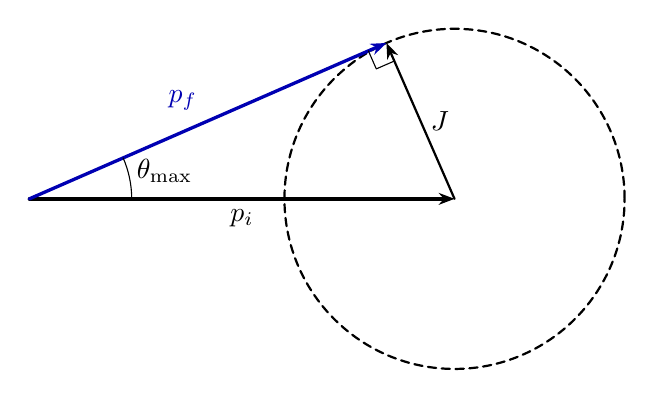
\begin{tikzpicture}[scale=0.9, line cap=round, line join=round, >={Stealth[length=2mm]}]
  \coordinate (O) at (0,0);
  \coordinate (C) at (6,0);
  \draw[thick, densely dashed] (C) circle (2.4);
  \draw[->, very thick] (O) -- (C) node[midway, below] {$p_i$};
  % tangent point: angle asin(2.4/6)
  \coordinate (T) at ({6*cos(23.58)*cos(23.58)},{6*cos(23.58)*sin(23.58)});
  \draw[->, very thick, blue!70!black] (O) -- (T) node[midway, above left] {$p_f$};
  \draw[->, thick] (C) -- (T) node[midway, right] {$J$};
  \pic[draw, "$\theta_{\max}$", angle radius=13mm, angle eccentricity=1.35] {angle = C--O--T};
  \pic[draw, angle radius=2.5mm] {right angle = O--T--C};
\end{tikzpicture}
\end{center}

\section*{Problem 25}
Read the question carefully: $\mu$ is between the block and the second ramp, so friction only applies to one. Set up energy and geometry and solve for $h_2$.

\end{document}
